% !TeX spellcheck = en_US
\chapter{Case studies}
\label{ch:cases}

We want to present two case studies with the aim of clarifying the concept of complicated decision problems and to understand the practical meaning fo the terminology presented earlier. 

Both case studies concern large public works and could undergo several variations and corrections, as they are not yet implemented.

\section{The tramway of Como}
\label{sec:comotram}

\subsection{Context}
\label{subsec:comocontext}

Como has been for centuries at the center of exchanges, connecting Italy to Switzerland and Germany, while being a connection to cities at the end of the alpine valleys (Varese, Lecco, Bergamo, etc.).

This favorable position has led to problems, mainly related to saturation of the access ways, with congestion, economic losses due to slow transfers, pollution and accidents as a result.

Private cars are the main responsible for these problems, they concentrate on a few relatively small streets, which can't be enlarged easily due to the orography of the site.

A possible improvement could be to use public transport, more efficient from a transportation capacity point of view. However, the fraction of transfers serviced by public transport is small, and very uneven. Buses service a minority of users and are subject to the same limitations as private cars. 

As for train services, the state railway is rather unloaded (FS line), while the regional railway is nearly saturated (FNM line). How can the capacity of the FNM line be increased? Maybe while moving some of its passenger on the FS line.

Some critical points to consider while discussing interactions among the lines: 
\begin{enumerate}
	\item The crossing between the lines occurs with an acrobatic system of bridge: the Napoleona street overcomes the FNM line, which overcomes the FS line, which overcomes a small local street (Via dei Mulini)
	
	\item Between the stations of Camerlata and Borghi, the FNM line has a single track, with steep slopes on both sides
	
	\item Between the stations of Borghi and Lago, the FNM line has a single track, running along a narrow alley between houses
	
	\item Joining the FS and FNM lines through the town plain would require first to cross either the walls (in a historical area) or along the lakefront (touristy, occupied by a main street and flooded from time to time), and then climb the steep slope on top of which lies the FS station of Como S. Giovanni
\end{enumerate}
 
All these factors make a solution based on railways impossible to adopt, unless limited to the use of existing tracks. Increasing the frequency of the trains on the FNM line, however, has two problems: 
\begin{itemize}
	\item The single-track line forbids two trains to run along the Camerlata-Borghi-Lago track (unless perfect synchronization, difficult and prone to big problems)
	
	\item The levels crossing cut the town in two for several minutes every time a train passes along them, which could lead to significant traffic congestion
\end{itemize}

Hence the idea of a tramway line, which could: 
\begin{itemize}
	\item Have a double track, thanks to the shorter gauge
	
	\item Have fast crossing with traffic lights, instead of slow level crossings
	
	\item Be prolonged to the inside of town
\end{itemize}

But a classical tramway involves a big problem, as it requires to replace the whole track, therefore 
\begin{itemize}
	\item forcing train passengers from outside Como to change at an external station
	
	\item completely blocking traffic during the works
\end{itemize}

\subsection{The generation of the alternatives}
\label{sec:comoalternatives}

In this case, the set of alternatives is far from being clear. More correctly, it is \textit{indefinite}, and must be built step by step by investigating the whole context. 

We need to follow the iterative approach defined in Section \ref{sec:modelingapproach}. For instance, if one realizes that modifying the gauge of the tracks is too expensive, one can wonder if there exists tramways able to use standard train tracks. \href{https://it.wikipedia.org/wiki/Tram-treno}{\texttt{They exist}}.

The process of generating alternatives becomes easier if one decomposes the problem, identifying the basic \textit{alternative elements}, which can be (at least partly) independent.

In this study, three fundamental elements have been identified, in order to base on them the generation of alternatives: 
\begin{enumerate}
	\item The technology used to implement the new line 
	
	\item The route of the new line
	
	\item The management of the FNM trains with respect to the new line
\end{enumerate}

\paragraph{Technology} Previous studies on similar cases suggest three possible technologies:
\begin{enumerate}
	\item Standard railway service: add a shuttle-train between Grandate e Como Lago, so as to increase the frequency of the current railway service
	
	\item Tramway: replace the railway with a classic tramway
	
	\item Interoperable: add to the current railway service a special tramway which is able to work with both systems (facing all the resulting problems)
\end{enumerate}

\paragraph{Route} The number of possible routes is huge and not well-defined \textit{a priori}. To start, four possible routes have been identified: 
\begin{enumerate}
	\item Keeping the current FNM route, ending at the station of Como Lago 
	
	\item Linking the station of Como Lago (FNM) to Como S. Giovanni (FS) through new tracks crossing the town center
	
	\item Linking the station of Como Lago (FNM) to Como S. Giovanni (FS) through new tracks passing along the lakeside
	
	\item Building a ring around the town center through a new track from Como Lago (FNM) to Como S. Giovanni, plus a track from Como S. Giovanni (FS) to Como Borghi (FNM)
\end{enumerate}

\paragraph{Management of the FNM trains} This element of the alternatives describes the relation between the two rail transportation systems:
\begin{enumerate}
	\item Keep the FNM service on its current route
	
	\item Move the FNM service to the FS station of Como S. Giovanni, through the construction of an interchange between the FNM and FS lines (probably in the station of Camerlata)
\end{enumerate}

These are extreme possibilities, with a range of intermediate solutions, either during the works or permanently.

Each of these aspects provides an \textit{alternative element}. The single possible choices for an element can be associated to numerical values: sometimes a proper quantitative measure, other times simple arbitrary indices (e.g., 0 for the railway, 1 for the tramway and 2 for the interoperable). The purpose of this association, in general, is to describe effectively the set of alternatives, not to make computations.

Once the elements of the alternatives and the possible values for each element have been identified, one can proceed to enumerate their combinations, which in general are not all feasible. In the present case  there are $3 \cdot 4 \cdot 2 = 24$ combinations, only 7 of which are feasible. The other ones can be excluded due to obvious contradictions, technical impossibility or common sense. 

For example, the railway technology is incompatible with any route different from the present one (trains cannot go through towns).

A fundamental remark on the generation of alternatives is that \textbf{there always exists an alternative that consists in doing nothing} and keeping the current situation, this is conventionally denoted as \textbf{alternative zero}. New alternatives should, at least, not worsen the current situation. This is far from trivial since \textit{"worsen"} is a complicated concept.

In this discussion, we have neglected several other potential elements of alternative, such as
\begin{itemize}
	\item The location of interchange parking (in various sites)
	
	\item The implementation of double-tracks rails along parts of the current single-track rail
	
	\item The construction of new stations along the current route and possible new routes
	
	\item Possible transfers of the current route
	
	\item The extension of the service out of Como, beyond the station of Grandate
	
	\item The frequency of the new service
	
	\item The tariffs of the new service
	
	\item \dots
\end{itemize}

In particular, some mobility studies suggest that there could be a strong request for a railway servicing parts of the province currently badly connected to Como, both eastward and westward. Other subsequent feasibility studies have focused on these aspects, rejecting the most extreme solutions (current route and town ring), merging the intermediate ones (center crossing and lakeside route) in a mixed variant.

We also neglected the possible \textit{mitigation measures}, all those interventions that must be added to the alternatives in order to correct the negative impacts they produce, or to convince stakeholders strongly opposing the project to accept it (or at least not fight it too much), or to modify the impact of the work (e.g. limited access zones to discourage private cars).

All this confirms that even listing the possible solutions of a decision problem can be a preliminary problem in itself, that is not to be solved in a single phase, and actually is never ultimately solved.

\subsection{The generation of scenarios}
\label{subsec:comoscenarios}

The generation of scenarios follows the same rationale as the generation of the alternatives, also requiring to predict events uncontrollable by the decision-makers. First, one identifies the \textit{scenario elements} and their possible values, then we consider only the feasible combinations. If new scenarios emerge, or old ones disappear, the study should be updated and corrected.

The scenario elements considered are the following ones: 
\begin{enumerate}
	\item Closure of the lakeside to private traffic: forbidding the access of vehicles to the street that runs between the city center and the lake, this interacts with the project as it frees up the space used by cars, making it easier to build a tramway along the lakeside
	
	\item International Como-Chiasso station: it consists of merging the international railway stations of Como (Italy) and Chiasso (Switzerland) in a single stop, half-way, accelerating the trips between Italy and central Europe, this interacts with the project because the station of Como S. Giovanni would be reduced to the level of local station, introducing the need for a service taking travelers to Como S. Giovanni and possibly onward to the new international station
	
	\item Anti-flood barriers: it consists of building barriers that protect the center of Como from lake floodings, this interacts because a tramway service passing along the lakeside would be blocked by floods
	
	\item Borgovico tunnel: a toll tunnel that should run from the north-west to the south-west of Como, allowing to cross the town without congesting the western side
	
	\item Underlake tunnel: a tunnel which should run under the lake to replace the street that currently connects the north-west and nort-east of Como
\end{enumerate}

In theory, each combination of these elements is possible, excluding combining the underlake tunnel with keeping the lakeside open (meaningless) and building both tunnels (too expensive).

This discussion neglects important aspects such as: 
\begin{itemize}
	\item The anticipated variations in the residential and economic structure of the area under study
	
	\item The variations in the \textit{origin-destination matrix (O/D matrix)} of the potential transportation demand (i.e., the number of trips from place to place that will take place in the town and could be captured by the new service)
	
	\item The amount of European, state and region financing
\end{itemize}

Some of these scenario correspond to predictable numerical values, while others correspond to event which can either occur or not, or could occur in different ways. 

For each numerical value, for each event or for each way in which an event can occur, it could be possible to estimate a probability, or at least provide a qualitative estimation of its likelihood. All this information concurs to describe the set of possible scenarios and its auxiliary information.

\subsection{The definition and computation of the indicators}
\label{subsec:comoindicators}

As the alternatives and the scenarios, also the impacts are combinations of different elementary quantities, which are usually named \textit{indicators}. They characterize the satisfaction of the decision-makers for a configuration of the system, and determine their preferences. Indicators are typically much more numerous and diversified that the elements of the alternatives and the scenarios, so numerous that their generation adopts a hierarchical process that progressively details the sectors of the impact: 
\begin{itemize}
	\item Identify general macrosectors
	
	\item Each macrosector is decomposed into sectors, and possibly into sub-sectors, progressively more specific
	
	\item The elementary indicators are identified
\end{itemize}

This mechanism produces an \textit{indicator tree}. 

In this case, the three standard macrosectors used in Environmental Impact Assessment (EIA) have been adopted:
\begin{enumerate}
	\item \textit{Environment}, subdivided into Air pollution, Noise, Vibrations, Landscape and Territorial structure (that is, the compatibility with the current management plans of the area)
	
	\item \textit{Economy}, subdivided into Costs, Revenues and House values
	
	\item \textit{Society}, subdivided into Appreciation, Discomfort, Accessibility, Employment, Induced effects
\end{enumerate}

but a fourth macrosector has been added
\begin{enumerate}
	\setcounter{enumi}{3}
	\item \textit{Transportation}, subdivided into Security, Congestion and Interferences
\end{enumerate}

This last one is usually included in the Society macrosector, but it has been attributed an autonomous role as the study evaluates a large transportation service.

This yields the indicator tree:
\begin{center}
	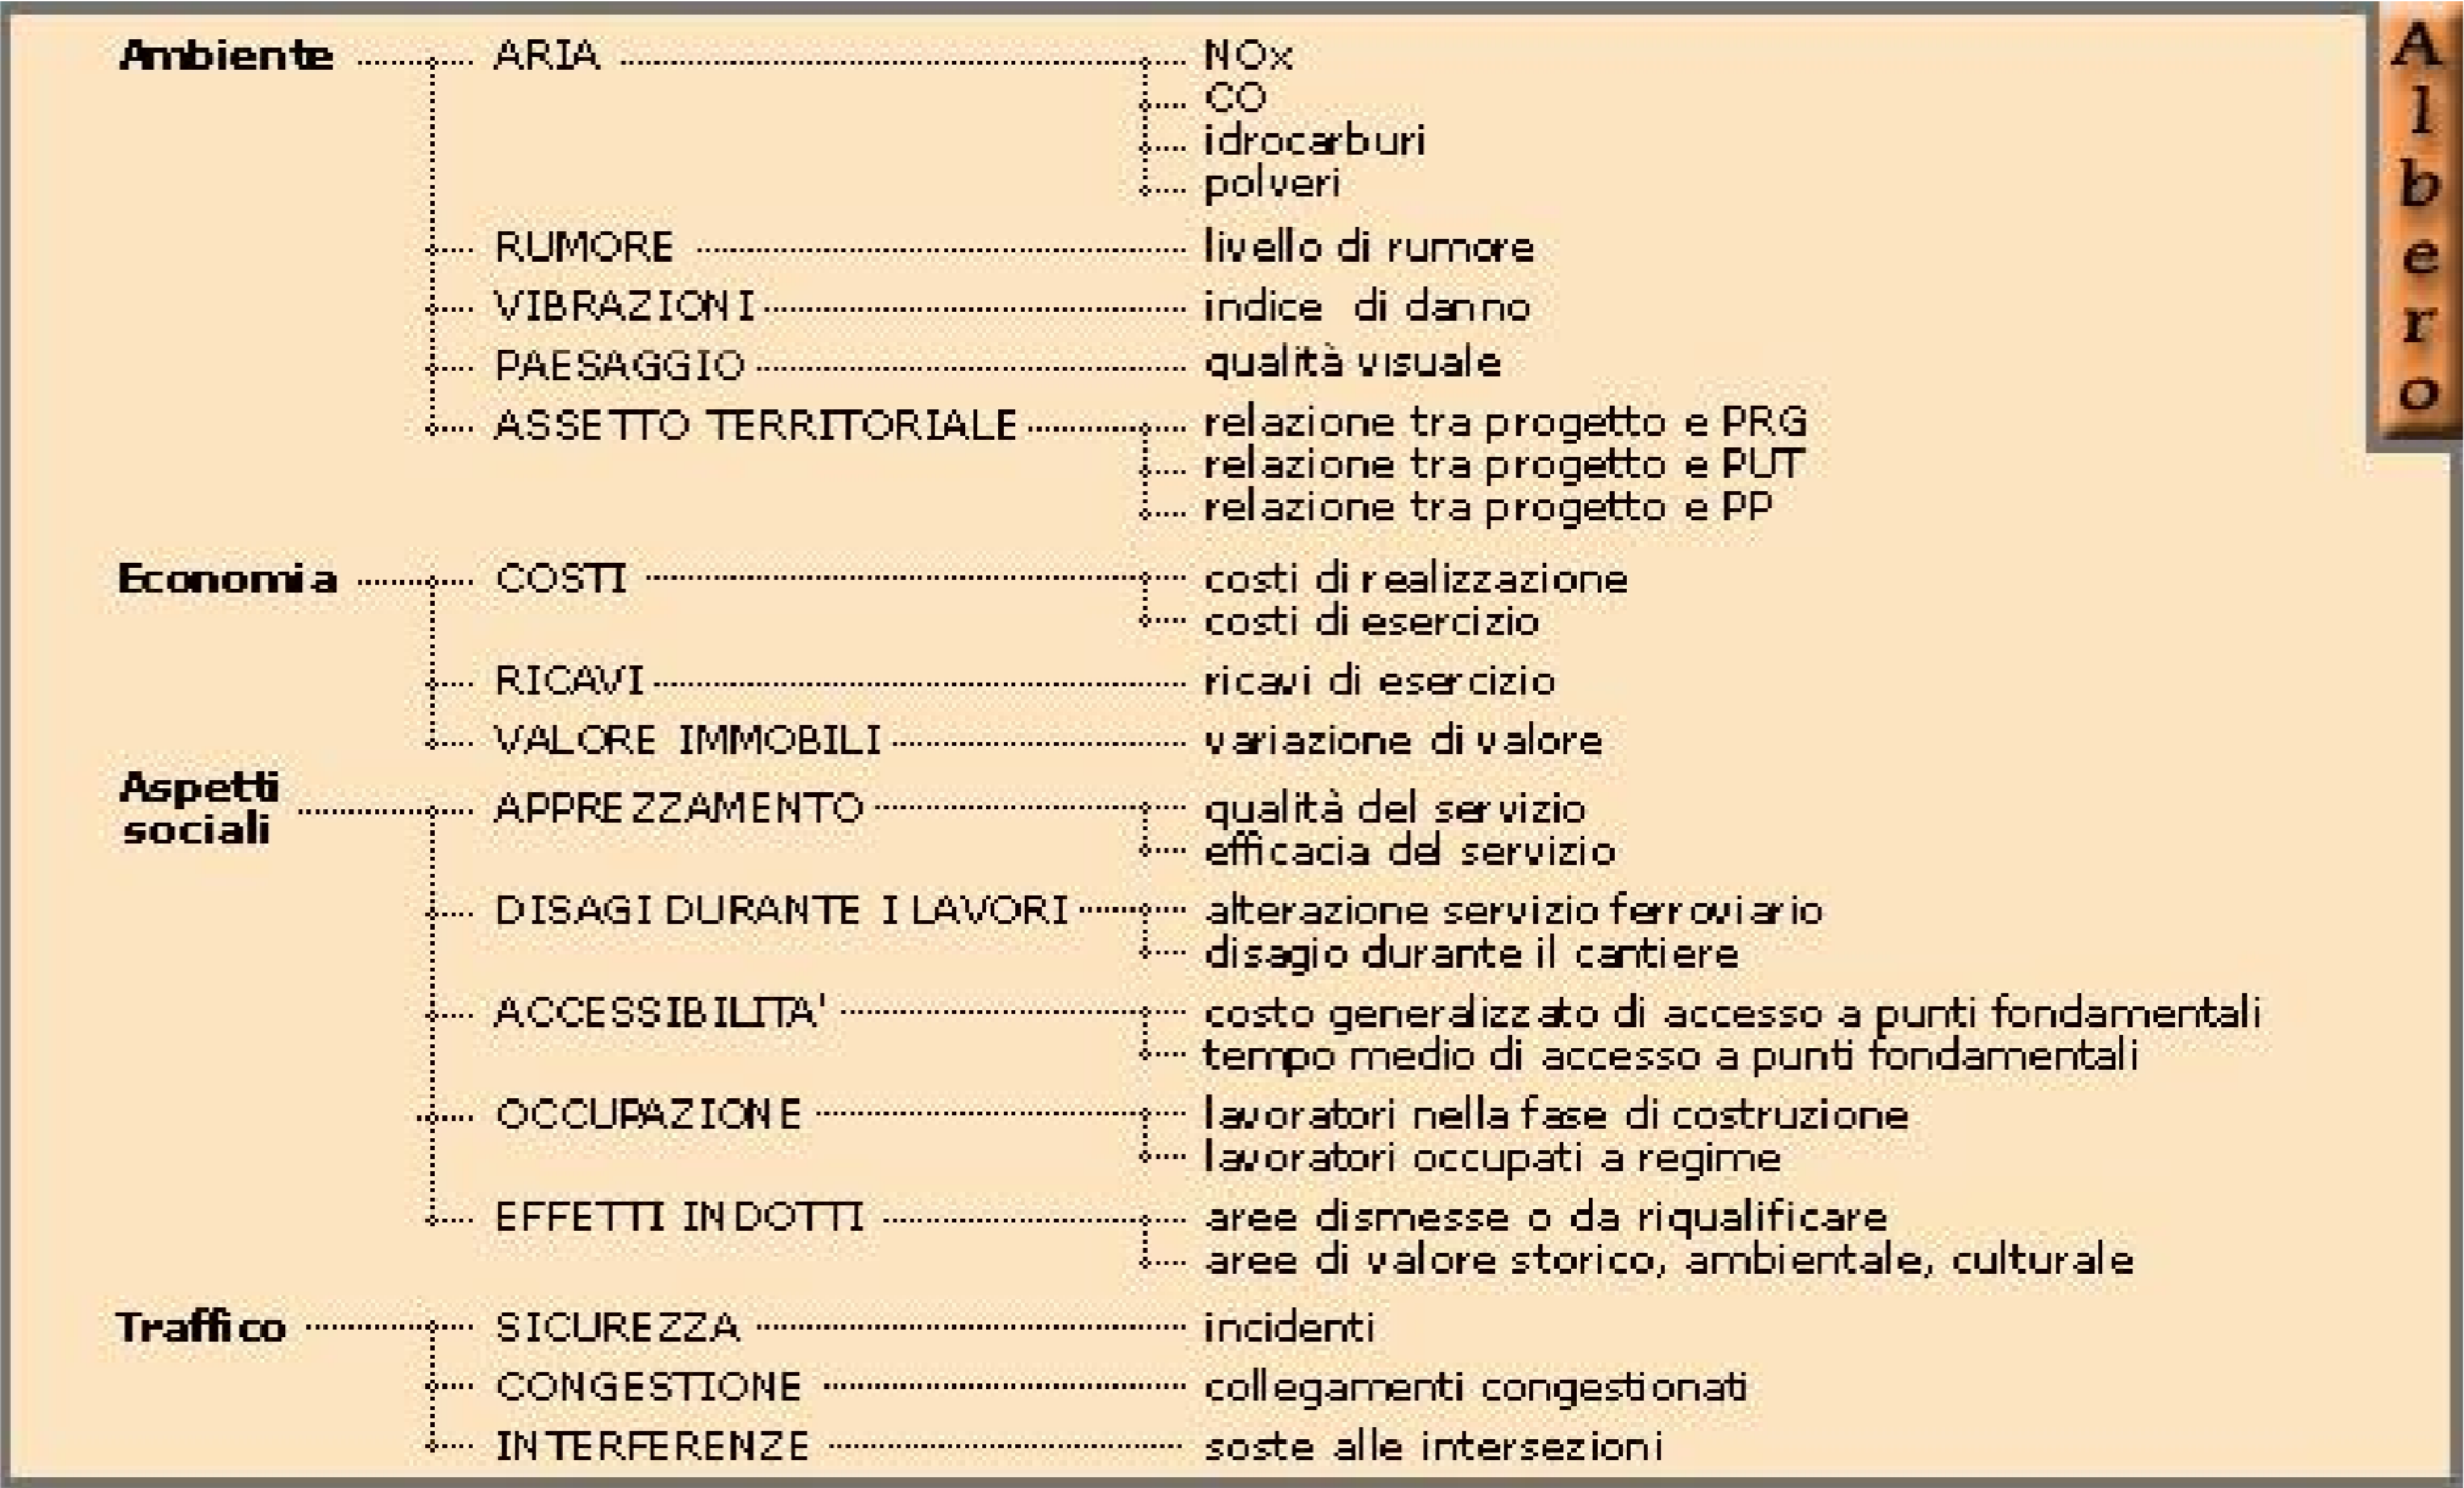
\includegraphics[width=0.98\columnwidth]{img/dp/cases/comotree}
\end{center}

The hierarchical structure aims to organize the evaluation of the single indicators during the phase of data collection; experts in each sector will be assigned to lead the estimation, prediction and measurement of the values of each indicator. 

Similarly, the construction of preferences in the decision phase will be organized based on the specific skills of experts of the various sectors; the "importance" of each indicator has to be determined.

Each indicator must be associated with a tool which will provide its values for each possible configuration. In most cases, these values will not be directly measurable, but are the result of estimates, given by a predictive model (e.g. $CO_2$ pollution can be measured now, but obviously not in all the hypothetical configurations).

The indicators can be numerical values that express physical measures, but also qualitative values on an ordinal scale. The purpose is not to make computations, just to describe the situation. In practice, some evaluation methods use such numerical values to make computations.

\paragraph{Time decomposition (phases) and space decomposition (zones)} Some indicators ave an intrinsic \textit{space} or \textit{time} feature, which must be taken into account; in other words, the values of an indicator might be meaningless if referred to the whole territory or whole time horizon of the project.

To correctly describe the situation, the system has to be divided into distinct geographical zones, on which is meaningful to define a value of the considered indicator.

This increases the amount of information to manage and requires to evaluate the relative importance of the different zones on the decision, as if they were values of different indicators. 

In this study, Como has been subdivided into 5 zones: 
\begin{itemize}
	\item Como centro 
	
	\item Borghi
	
	\item Camerlata
	
	\item Lora 
	
	\item Tavernola
\end{itemize}

Only the first three zones are directly affected by the project, whereas Lora and Tavernola have been maintained to check indirect effects on the whole town.

\subsection{The definition of the stakeholders}
\label{subsec:comostakeholders}

We denote as \textit{stakeholders} every person, organization, category or institution that is involved, directly or indirectly, in the project, even if it plays no role in the decision, since its interests are affected by the project.

The fundamental aspect in the description of stakeholders is to characterize their \textit{preferential structure}. However, the stakeholders could also point out neglected alternatives, scenario elements and indicators.

For this case, four classes of stakeholders have been identified: 
\begin{enumerate}
	\item Institutional stakeholders (Municipality, Province, Region)
	
	\item Society
	\begin{itemize}
		\item Citizens
		
		\item Environmentalists associations
		
		\item Category associations
	\end{itemize}
	
	\item Users
	\begin{itemize}
		\item Regular (commuters, students, etc.)
		
		\item Irregular
	\end{itemize}
	
	\item Transportation companies 
	\begin{itemize}
		\item FNM, whose track between Grandate and Como Lago should be used by the new service
		
		\item SPT, the local public transport company managing the bus lines, whose demand would be disrupted by the new service, requiring revision of routes and schedules
		
		\item FS, whose station of Como S. Giovanni could host part or all the trains currently servicing the FNM line
	\end{itemize}
\end{enumerate}

Each stakeholder has limited interests and skills, often related to one or few subtrees of the indicator tree, hence it will usually be involved mainly in the phases of the decision process which concerns those specific indicators. 

For this case, the relation between stakeholders and subsectors:
\begin{enumerate}
	\item The local government stakeholders will be interested in the whole system of indicators
	
	\item Concerning society stakeholders: 
	\begin{itemize}
		\item The citizen will probably focus their interest on the Environment, Society and transportation macrosectors
		
		\item The environmental associations will focus on the environmental macrosector
		
		\item The category associations (Camera di Commercio, Industria, Artigianato e Agricoltura, Confesercenti, \dots), who support the economic interests of the traders and entrepreneurs, will focus on the Economy macrosector and on the discomfort introduced by the works
	\end{itemize}
	
	\item The users will focus on the society macrosector, in particular on quality and accessibility of the service
	
	\item Concerning the transport companies
	\begin{itemize}
		\item FNM will focus on the Society (Emplyment and Discomfort) and Economy (Costs and Revenues) macrosectors
		
		\item SPT will focus on Society, Economy and Transportation macrosectors (Emplyment, Discomfrot, Traffico congestion and its own Costs and Revenues)
		
		\item FS is interested in the management of the train service potentially moved to the station of Como S. Giovanni
	\end{itemize}
\end{enumerate}

Once stakeholders have been identified, a reference person (or group) should be defined for each stakeholder, and involved in all phases of the decision process and subsequent iterations. 

The tools to interact with the person depend on the specific group of stakeholders considered; such tools could be talking with representatives of the group or polls, forms and interviews to the relevant subjects.

Some group of stakeholders can partly overlap (e.g. environmentalists and shopkeepers are also citizens), but the preference of common citizens will be different from those of a specific group, making it correct to represent them as different stakeholders.

\subsection{The decision process}
\label{subsec:comodecisionprocess}

For each possible configuration of the system it's necessary to evaluate each indicator, sometimes requiring physical measurements, but most of the time a suitable descriptive model can be applied to compute the expected value. Speaking in qualitative terms:
\begin{itemize}
	\item The alternatives exploiting the railway technology will have
	\begin{itemize}
		\item low implementation costs and low discomfort
		
		\item limited effect on the accessibility of sites not currently serviced
		
		\item limited environmental improvements
		
		\item nearly no impact on the employment
		
		\item \dots
	\end{itemize}
	
	\item The alternatives exploiting the "interoperable" technology will have
	\begin{itemize}
		\item higher economic costs
		
		\item stronger penetration of the service in the urban fabric, dependent on the chosen route
		
		\item intermediate discomfort
		
		\item \dots
	\end{itemize}
	
	\item The alternatives exploiting the classical tramway technology will have
	\begin{itemize}
		\item much higher implementation costs and times
		
		\item very detailed service
		
		\item \dots
	\end{itemize}
\end{itemize}

The resulting numerical and qualitative values will have to be aggregated depending on the preferences of the various stakeholders. It's necessary to model the preferential structure of each stakeholder, to determine preference among different impacts.

It is also necessary to aggregate the preferences of different stakeholders in a final ordering of the alternatives, or at least in the selection of one alternative. The \textit{sensitivity} of the final ordering should also be taken into account, that is the boundaries within which it remains valid when the data changes.

\section{Reopening of the Navigli in Milan}
\label{sec:navi}

\subsection{The context}
\label{subsec:navicontext}
Milan was born as a river town, rich in natural rivers, later further enriched by a network of canals. Modernity led to covering the whole network in favor of traffic and, more recently, to a periodic proposal and discussion of project to reopen part of it.

The main motivations for the project are:
\begin{itemize}
	\item The \textit{hydraulic continuity}, that is the possibility to better control and limit the flooding of water streams in the northern part of Milan, currently flowing through pipes, limiting the capacity and making cleansing more difficult
	
	\item The \textit{touristic and commercial navigability}, with their social, cultural and economic outcomes
	
	\item The \textit{production of electricity}, not by directly installing turbines in the Navigli, but with the increase of water flow in the Naviglio Pavese, which has several small hydroelectric plants south of Milan
	
	\item The \textit{feeding of heat-pump plants} in the area of Darsena using nappe (underground) water
	
	\item The \textit{decrease in the nappe level}, thanks to the extraction of water from wells which are currently closed, reducing the use of pumps in several underground stations that defend the tunnels from flooding
\end{itemize}

\subsection{The definition of the alternatives}
\label{subsec:navialternatives}

The definition of alternatives seems easier in this case, given the Navigli's well defined historical route. In practice, things are not easy.

Starting from a basic dichotomy, one can distinguish: 
\begin{itemize}
	\item "Virtual" alternatives, in which the Navigli are not actually reopened, but made enjoyable with public visual aids (sings, pavings, \dots)
	
	\item "Physical" alternatives, in which the Navigli are actually reopened
\end{itemize}

All physical alternatives do not share the same route, there are many alternatives: 
\begin{itemize}
	\item A partial reopening, keeping some covered stretches
	
	\item A complete reopening of the classic circle north-east-south, which includes a number of minor variations concerning
	\begin{itemize}
		\item Porta Nuova park
		
		\item Cavour Square
		
		\item the Vallone Naviglio
		
		\item the Viarenna basin
	\end{itemize}
	
	\item The reopening og the whole inner circle, also on the western side: some technical reasons make this alternative quite impractical (mainly, it interferes with underground line 2)
	
	\item Additional works with respect to the historical route:
	\begin{itemize}
		\item the Vettabbia canal
		
		\item the "Darsena 2" project, a brand new basin near the railway station Porta Genova
	\end{itemize}
\end{itemize}

Another fundamental element of the alternatives is navigability: the new canal could be open or closed to boat trips. The elements of alternative (route, navigability and other possible ones) must then be combines to build the alternatives, removing impossible combinations (virtual alternatives obviously forbid navigability).

\subsection{The definition of the scenarios}
\label{subsec:naviscenario}

This point is not developed in the project described, we therefore make a superficial analysis. The fundamental aspects of the scenario are:
\begin{itemize}
	\item Availability of public funding to build and manage the canal
	
	\item The (more or less) strict closure of the city center to private cars
	
	\item The construction of underground line 4 (completed as of writing) which would provide easy access on foot to most of the city center, even if private cars and some bus lines could not access it
\end{itemize}

\subsection{The definition and computation of the indicators}
\label{subsec:naviindicators}

We, once again, proceed in a hierarchical way, to identify large sectors and then dividing them. To give a non-exhaustive list:
\begin{itemize}
	\item Impact on pollution
	
	\item Variation of travel times to various parts of town
	
	\item Impact on traffic congestion
	
	\item Impact on public transport
	
	\item Construction costs
	
	\item The hedonic impact on the real estate prices
	
	\item Impact on commercial activities
\end{itemize}

Some of these impacts could be so negative as to introduce a feedback loop on the definition of the alternatives, a correction and update of the alternatives through the introduction of devices to reduce those impacts. E.g. bridges used by tramway can't have slopes, which implies a water level low enough and boat suitably designed in order to allow navigability.

\subsection{The time and space organization}
\label{subsec:navitimespace}

Several indicators are naturally related to geographical positions. Some indicators refer to zones, whereas others to linear stretches of the Naviglio. The detailed project divides the route of the canal into 16 stretches.

Concerning the time phases, some of them correspond, somehow, to alternatives, meaning it's  possible to implement a specific phase then leave the following "frozen" for a long time, waiting for favorable conditions to complete them. For example, virtual alternatives can be seen as a preliminary phase to a global reopening. They could achieve a partial result at low cost, however they could increase the overall cost.


The construction of a double Naviglio, with an underground pipe running under the canal is an additional cost, but it also allows to reach in short time the result of hydraulic continuity and to spread over time the following phases, dividing the expense.

\subsection{The definition of the stakeholders}
\label{subsec:navistakeholders}

The definition of the stakeholders is similar to what described in for the tramway of Como (\ref{subsec:comostakeholders}). The mayor of Milan can be considered as the decision-maker, but other subjects must be taken into account, such as transportation companies (mainly ATM, railway lines are not affected), the environmental and category associations, citizens. Among the citizens, the owners of real estate along the route of the canal could be considered specifically.

\subsection{The decision process}
\label{subsec:navidecision}

Once again, it's necessary to evaluate each indicator in each possible configuration. This implies the application of suitable descriptive models. One could expect that
\begin{itemize}
	\item The "virtual" alternatives will be particularly cheap and have negligible impact on traffic and pollution, but will not offer any advantage with respect to hydraulic continuity (unless combined with the construction of an underground pipe), to the production of electricity and to the management of water nappe, and they have limited impact on tourism and commerce; the aesthetic impact is harder to evaluate
	
	\item The "physical" alternatives will be much more expensive, reaching the objective of hydraulic continuity, electricity production, management of water nappe, while favoring tourism, commerce, real estate prices and aesthetic impact
\end{itemize}

Moreover
\begin{itemize}
	\item The alternatives involving a navigable canal will have touristic, commercial and accessibility advantages, but at a higher cost, requiring to manage a system of gatehouses to get over the height difference between subsequent stretches of the canal
	
	\item The alternatives involving a non-navigable canal will be cheaper, but less advantageous for accessibility, commerce and tourism, even if they could have a better aesthetic impact, since a navigable canal requires a relatively low water level to let boats pass under bridges
\end{itemize}

After all indicators have been evaluated, the aggregation phase can start, taking into account the preferential structure of all the stakeholders. This can be done in several ways and should conclude with an ordering of the alternatives, or at least the choice of one, also with the information on the sensitivity on such an ordering or choice.

% This should be L2
